% Created 2018-11-25 Sun 11:13
% Intended LaTeX compiler: pdflatex
\documentclass[presentation]{beamer}
\usepackage[utf8]{inputenc}
\usepackage[T1]{fontenc}
\usepackage{graphicx}
\usepackage{grffile}
\usepackage{longtable}
\usepackage{wrapfig}
\usepackage{rotating}
\usepackage[normalem]{ulem}
\usepackage{amsmath}
\usepackage{textcomp}
\usepackage{amssymb}
\usepackage{capt-of}
\usepackage{hyperref}
\usepackage{etex}
\usepackage{amsmath}
\usepackage{pgfplots}
\usepackage{tikz}
\usepackage[europeanresistors,americaninductors]{circuitikz}
\usepackage{colortbl}
\usepackage{yfonts}
\usetikzlibrary{shapes,arrows}
\usetikzlibrary{positioning}
\usetikzlibrary{arrows,shapes}
\usetikzlibrary{intersections}
\usetikzlibrary{calc,patterns,decorations.pathmorphing,decorations.markings}
\usepackage[BoldFont,SlantFont,CJKchecksingle]{xeCJK}
\setCJKmainfont[BoldFont=Evermore Hei]{Evermore Kai}
\setCJKmonofont{Evermore Kai}
\AtBeginSection[]{\begin{frame}<beamer>\frametitle{Topic}\tableofcontents[currentsection]\end{frame}}
\setbeamercovered{transparent}
\usetheme{default}
\date{}
\title{补充例子}
\hypersetup{
 pdfauthor={},
 pdftitle={补充例子},
 pdfkeywords={},
 pdfsubject={},
 pdfcreator={Emacs 26.1 (Org mode 9.1.9)}, 
 pdflang={English}}
\begin{document}

\maketitle
\begin{frame}{Outline}
\tableofcontents
\end{frame}




\section{关于反馈}
\label{sec:org223d099}
\begin{frame}[label={sec:org4009c8c}]{反馈与方程(静态)}
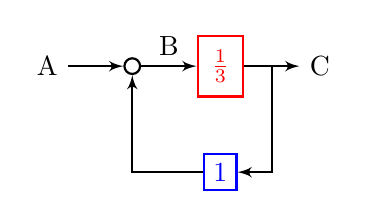
\begin{tikzpicture}[node distance=2em,auto,>=latex', thick]
%\path[use as bounding box] (-1,0) rectangle (10,-2); 
\path[->] node[] (r) {A}; 
\path[->] node[ circle,inner sep=2pt,minimum size=1pt,draw,label=below left:$ $,right =of r] (p1) { }; 
\path[->](r) edge node {} (p1) ; 
\path[red] node[draw, inner sep=5pt,right =of p1] (g) {$\frac{1}{3}$}; 
\path[->] (p1) edge node[midway] {B} (g) ; 
\path[->] node[ right =of g] (o) {C}; 
\path[->] (g) edge node {} (o); 
\path[blue] node[draw, below =of g] (h) {1};
\path[->,draw] (g.east)+(1em,0) |- (h.east) ; 
\path[->,draw] (h.west) -| (p1) ; 
\end{tikzpicture} 

\begin{eqnarray}
C &=& \frac{B}{3}\\
A+C &=& B\\
A &=& 10\\
C &=& ?
\end{eqnarray}
\end{frame}

\begin{frame}[label={sec:org66a2ef4}]{笑话:过桥}
路人甲要过桥,发现桥很长,问桥边路人乙桥长多少,乙说:50米。甲走上桥后不一会儿,乙追了上来,说,桥长100米,你要是过了50米就转弯,就掉下去了。

\begin{center}
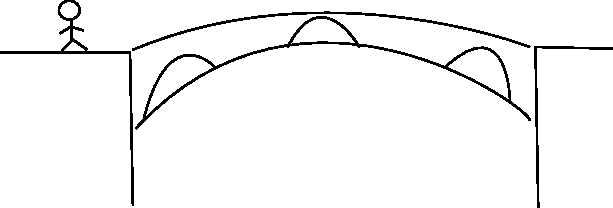
\includegraphics[width=.9\linewidth]{image/bridge.pdf}
\end{center}
\end{frame}

\begin{frame}[label={sec:org5ae0730}]{开环控制:笑话:不听话的儿子}
\end{frame}
\begin{frame}[label={sec:orgf2b2e52}]{开环控制:声东击西}
\end{frame}
\begin{frame}[label={sec:org1d9eb23}]{操纵杆}
飞行员拉动操纵杆,飞机机头上扬,结果减弱了拉动操纵杆的效果,即:拉杆->A增大->机头上扬->A减小

\begin{center}
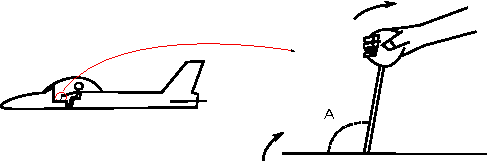
\includegraphics[width=.9\linewidth]{image/pilot.pdf}
\end{center}
\end{frame}

\begin{frame}[label={sec:org8103461}]{油门、刹车}
司机踩刹车,汽车减速,司机因为惯性会有前冲的趋势,易导致踩刹车的力度变大。

司机踩油门,汽车加速,司机因为惯性会有后仰的趋势,易导致踩油门的力度变小。

\begin{center}
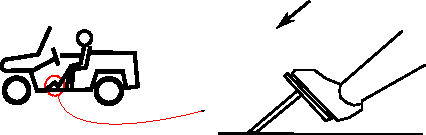
\includegraphics[width=.9\linewidth]{image/drive.pdf}
\end{center}
\end{frame}

\section{非线性}
\label{sec:org425e4ac}
\begin{frame}[label={sec:orga66f575}]{几个例子}
\begin{align*}
c &= u\\
c &= u+1\\
c &= 1\\
c &= 0\\
c &= \sqrt[3]{u} \quad u= x^3 \\
c+c^2 &= u \quad u=r+c^{2}
\end{align*}
\end{frame}
\begin{frame}[label={sec:org7e4983a}]{\(x'+1 =u\)}
\begin{columns}
\begin{column}{0.5\columnwidth}
\begin{block}{方法1}
变量代换,为方程右边与输出变量无关的部分指定另一个变量。
\begin{align*}
x'+1 &= u \\
w &= u-1 \\
x' &= w 
\end{align*}
\end{block}
\end{column}

\begin{column}{0.5\columnwidth}
\begin{block}{方法2}
将方程右边与输出变量无关的部分用泰勒级数展开。
\begin{align*}
x' &=u-1 \\
u-1 &= (u-1)|_{u=1}+\Delta u \\
x' &= \Delta u 
\end{align*}
\end{block}
\end{column}
\end{columns}
\end{frame}
\begin{frame}[label={sec:org3f18657}]{\(cc'=u\)}
\begin{columns}
\begin{column}{0.5\columnwidth}
\begin{block}{在 \(c_0=1,c'_0=1\) 处线性化}
\begin{align*}
(1+\Delta c)(1+\Delta c') &= u \\
1+\Delta c+ \Delta c' + \Delta c \Delta c' &= u\\
\Delta c +\Delta c' &= \Delta u
\end{align*}
\(\Delta u=0,u=1\) 时, \(cc'=1\) 。接着随着 \(c\) 增大,\(c'\) 会减小。
\end{block}
\end{column}

\begin{column}{0.5\columnwidth}
\begin{block}{变量代换 \(c=t+\Delta c,c'=1+\Delta c'\)}
\begin{align*}
(t+\Delta c)(1+\Delta c') &=u \\
t+\Delta c+t\Delta c'+\Delta c\Delta c' &=u \\
\Delta c+t\Delta c'+\Delta c\Delta c' &=u-t \\
\Delta c +t\Delta c' &= \Delta u
\end{align*}
\(\Delta u=0,u=t\) 时, \(cc'=t\) 。接着随着 \(c\) 增大,\(c'\) 不变。
\end{block}
\end{column}
\end{columns}
\end{frame}
\section{稳定性}
\label{sec:orgc3b912b}
\begin{frame}[label={sec:org8718970}]{稳定性与平衡点}
\begin{eqnarray*}
\dot x(t)-x(t) & = & r(t)\\
r &=& 1 \\
x(0) &=& -1 \\
x(t) &=& -1
\end{eqnarray*}

\begin{itemize}
\item 通解:$x_1(t)=a_0e^t$
\item 特解:$x_2(t)=-1$
\item $x_1(0)+x_2(0)=x(0)$得$a_0=0$
\end{itemize}
\end{frame}

\begin{frame}[label={sec:orgcbe1435}]{信号、系统、零极点相消}
考虑两种情况:

\begin{itemize}
\item \(G(s)=\frac{s-1}{s+1},R(s)=\frac{1}{s-1}\)
\item \(G(s)=\frac{1}{s-1},R(s)=\frac{s-1}{s+1}\)
\end{itemize}

系统初始值为0时,可得:\(C(s)=G(s)R(s)=\frac{1}{s+1}\)
当系统存在初始值 \(y_0\) 时,则分别变为

\begin{itemize}
\item \(C(s)=\frac{y_0}{s+1}+\frac{1}{s+1}\)
\item \(C(s)=\frac{y_0}{s-1}+\frac{1}{s+1}\)
\end{itemize}
\end{frame}

\begin{frame}[label={sec:org989224a}]{终值定理、稳态响应、直流分量}
终值定理计算的是瞬态响应消失后稳态响应中的直流分量,可以结合Fourier变换分析。
\begin{align*}
\lim_{s\to 0}sC(s) &= \lim_{s\to 0}G(s)R(s) \\
\lim_{\omega\to 0}C(j\omega) &= \lim_{\omega\to 0}G(j\omega)R(j\omega)\\
\end{align*}
从终值定理的证明过程(用到微分性质 \({\cal L}[\frac{df(t)}{dt}]=sF(s)-f(0)\) ,两边对 \(s\to 0\) 取极限)也可以看出,对于 \(f(t)=e^{\lambda t}\) ,
\begin{align*}
\lim_{s\to 0}{\cal L} [\frac{df(t)}{dt}]&=\lim_{s\to 0}\frac{\lambda}{s-\lambda}=
\begin{cases}
-f(0)  & \lambda\neq 0\\
0   & \lambda=0
\end{cases}\\
\lim_{s\to 0} sF(s) &=
\begin{cases}
0  & \lambda\neq 0\\
f(0)   & \lambda=0
\end{cases}
\end{align*}
即:对于 \(e^{\lambda t},(\lambda\neq0)\) 的分量,无论 \(\lambda>0,\lambda<0\) 利用终值定理计算时均为0。
\end{frame}
\begin{frame}[label={sec:org011e609}]{正反馈与离散系统稳定性}
\begin{eqnarray*}
x(n+1)-kx(n) &=& r(n) \\
r(n) & = & 0 \\
x(n) &=& x(0)k^n
\end{eqnarray*}
\end{frame}

\begin{frame}[label={sec:orgeb08067}]{正反馈与延迟系统稳定性}
\begin{eqnarray*}
x(t+a)-kx(t) &=& r(t) \\
r(t) &=& 0 \\
x(na) &=& x(0)k^{n}
\end{eqnarray*}
\end{frame}

\section{卷积}
\label{sec:org38f146c}
\begin{frame}[label={sec:orgd517f99}]{卷积与脉冲响应}
\begin{itemize}
\item 卷积
\begin{eqnarray*}
x(t)*y(t) &=& \int_{-\infty}^{\infty}x(\tau)y(t-\tau)d\tau \\
x(t)*\delta(t)& = & x(t) \\
\end{eqnarray*}
\end{itemize}
\begin{itemize}
\item 脉冲响应
设线性时不变(Linear Time Invariant,LTI)系统脉冲响应为 \(h(t)\) :
\begin{eqnarray*}
h(t) &=& LTI[\delta(t)]\\
h(t-\tau) &=& LTI[\delta(t-\tau)]\\
\end{eqnarray*}
\end{itemize}
\end{frame}

\begin{frame}[label={sec:org3fe28b0}]{卷积与系统响应}
设输入信号为 \(x(t)\) 时,输出为 \(y(t)\) :
\begin{eqnarray*}
y(t) & =& LTI[x(t)]\\
     &=& LTI\left[\int_{-\infty}^{\infty}x(\tau)\delta(t-\tau)d\tau\right] \\
     &=& \int_{-\infty}^{\infty} LTI[x(\tau)\delta(t-\tau)]d\tau \\
     &=& \int_{-\infty}^{\infty} x(\tau)LTI[\delta(t-\tau)]d\tau \\
     &=& \int_{-\infty}^{\infty} x(\tau) h(t-\tau)d\tau \\
     &=& x(t) * h(t)
\end{eqnarray*}
\end{frame}

\section{误差}
\label{sec:orgaad6672}
\begin{frame}[label={sec:orgdc24fc9}]{阶跃输入}
\begin{eqnarray*}
 m \dot{v} & =& f\\
 m \dot{v} & =& r-v\\
 m \dot{v} & =& 1-v\\
 m \frac{d}{dt}(v-1) & =& 1-v\\
 m \frac{d}{dt}(1-v) & =& -(1-v)\\
m \dot{E} &=& -E \\
E &=& e^{-\frac{t}{m}}
\end{eqnarray*}
\end{frame}

\begin{frame}[label={sec:orgaf5f3c2}]{斜坡输入}
\begin{eqnarray*}
 m \dot{v} & =& f\\
 m \dot{v} & =& r-v\\
 m \dot{v} & =& t-v\\
 m \frac{d}{dt}(v-t) +m & =& t-v\\
 m \frac{d}{dt}(t-v) & =& -(t-v) +m\\
m \dot{E} &=& -E +m\\
E &=& (1-m)e^{-\frac{t}{m}}+m
\end{eqnarray*}
\end{frame}

\section{Fourier变换}
\label{sec:orgefb0c49}
\begin{frame}[label={sec:org259d6b1}]{Fourier级数(三角形式)}
\begin{eqnarray*}
f_T(t) & =& \frac{a_0}{2}+\sum_{n=1}^{\infty}(a_n\cos(n\omega t)+b_n\sin(n\omega t))  
\end{eqnarray*}
其中:
\begin{eqnarray*}
\omega & =& \frac{2\pi}{T}\\
a_0 &=& \frac{2}{T}\int_{-\frac{T}{2}}^{\frac{T}{2}}f_T(t)dt \\
a_n &=& \frac{2}{T}\int_{-\frac{T}{2}}^{\frac{T}{2}}f_T(t)\cos(n\omega t)dt \\
b_n &=& \frac{2}{T}\int_{-\frac{T}{2}}^{\frac{T}{2}}f_T(t)\sin(n\omega t)dt \\
\end{eqnarray*}
\end{frame}

\begin{frame}[label={sec:org7b45a7e}]{Fourier级数(复指数形式)}
\begin{eqnarray*}
f_T(t) & = & \sum_{n=-\infty}^{+ \infty}c_n e^{j\omega_n t} \\
f_T(t) & = & \frac{1}{T}\sum_{n=-\infty}^{+\infty}\left[ \int_{- \frac{T}{2} }^{\frac{T}{2}}f_T(\tau)e^{-j\omega_n\tau}d\tau\right] e^{j\omega_n t} 
\end{eqnarray*}
\end{frame}
\begin{frame}[label={sec:org03c8c53}]{Fourier积分}
\begin{eqnarray*}
\lim_{T\rightarrow+\infty}f_T(t) &=& f(t) \\
f(t) & = & \lim_{T\rightarrow+\infty}\frac{1}{T}\sum_{n=-\infty}^{+\infty}\left[ \int_{- \frac{T}{2} }^{\frac{T}{2}}f_T(\tau)e^{-j\omega_n\tau}d\tau\right] e^{j\omega_n t} \\
\Delta\omega &=& \frac{2\pi}{T} \\
f(t) & = & \lim_{\Delta\omega\rightarrow 0}\frac{1}{2\pi}\sum_{n=-\infty}^{+ \infty}\left[ \int_{- \frac{T}{2} }^{\frac{T}{2}}f_T(\tau)e^{-j\omega_n\tau}d\tau\right] e^{j\omega_n t}\Delta\omega \\
f(t) & = & \frac{1}{2\pi}\int_{-\infty}^{+\infty}\left[ \int_{-\infty }^{\infty}f(\tau)e^{-j\omega\tau}d\tau\right] e^{j\omega t}d\omega
\end{eqnarray*}
\end{frame}
\begin{frame}[label={sec:orga2246bc}]{Fourier变换定义}
\begin{eqnarray*}
f(t)& = &\frac{1}{2\pi}\int_{-\infty}^{+\infty}\left[ \int_{-\infty }^{\infty}f(\tau)e^{-j\omega\tau}d\tau\right]e^{j\omega t}d\omega \\
F(j\omega)&=& \int_{-\infty}^{ + \infty}f(t)e^{-j\omega t}dt \\
f(t)  & =& \frac{1}{2\pi} \int_{-\infty}^{+\infty}F(j\omega)e^{j\omega t}d\omega \\
F(j\omega) &=& {\cal F}[f(t)] \\
f(t) &=& {\cal F}^{-1}[F(j\omega)] 
\end{eqnarray*}
\end{frame}
\begin{frame}[label={sec:org972f274}]{常用函数的Fourier变换}
\begin{itemize}
\item 单位脉冲函数 \(f(t)=\delta(t) \rightarrow   F(j\omega)=1\)
\item 阶跃函数 \(f(t)=A,(t\geq 0) \rightarrow   F(j\omega)=\pi\delta(\omega)+\frac{1}{j\omega}\)
\item 指数函数 \(f(t)=e^{at},(t\geq 0) \rightarrow  F(j\omega)=\frac{1}{j\omega-a}\)
\item 正弦函数 \(f(t)=\sin(\omega_0 t)\rightarrow F(j\omega)=\pi[\delta(\omega+\omega_0)+\delta(\omega-\omega_0)]\)
\end{itemize}
\end{frame}
\begin{frame}[label={sec:orge0cd198}]{性质}
\begin{itemize}
\item 线性: \(f(t)=af_1(t)+bf_2(t)\rightarrow  F(j\omega)=aF_1(j\omega)+bF_2(j\omega)\),其中 \(a,b\) 为常数
\item 时移: \(g(t)=f(t\pm a) \rightarrow  G(s)=F(j\omega)e^{\pm j\omega a}\)
\item 频移:\({\cal F}[e^{\pm\omega_0 t}f(t)]=F(j(\omega\mp\omega_0))\)
\item 时域微分: \(g(t)=f(t)'\rightarrow  G(j\omega)=j\omega F(j\omega)\)
\item 频域微分:\({\cal F}[tf(t)]=j\frac{dF(j\omega)}{d\omega}\)
\item 时域积分: \(g(t)=\int_{-\infty}^{t} f(\tau) d\tau \rightarrow  G(j\omega)=\frac{F(j\omega)}{j\omega}+\pi F(0)\delta(\omega)\)
\item 卷积:\({\cal F}[f_1(t)*f_2(t)]={\cal F}[f_1(t)]{\cal F}[f_2(t)]\)
\end{itemize}
\end{frame}

\section{连续系统频域分析}
\label{sec:org1009614}
\begin{frame}[label={sec:orgcabe151}]{基本信号 \(e^{j\omega t}\) 通过线性系统}
\begin{eqnarray*}
f(t) & =& e^{j\omega t},\qquad -\infty < t < \infty \\
H(j\omega) &=& \int_{-\infty}^{\infty}h(t)e^{-j\omega t}dt \\
           &=& |H(j\omega)|e^{j\phi(\omega)} \\
y_f(t) &=& e^{j\omega t}*h(t) \\
       &=& \int_{-\infty}^{\infty}h(\tau)e^{j\omega(t-\tau)}d\tau \\
       &=& e^{j\omega t}\int_{-\infty}^{\infty}h(\tau)e^{-j\omega\tau}d\tau \\
       &=& H(j\omega)e^{j\omega t} \\
       &=& |H(j\omega)|e^{j(\omega t+\phi(\omega))}
\end{eqnarray*}
\end{frame}
\begin{frame}[label={sec:orga360b06}]{正弦(余弦)信号通过线性系统}
\begin{eqnarray*}
f(t) & =& A\cos\omega t , \qquad  -\infty<t<\infty \\
     &=&\frac{A}{2}(e^{j\omega t}+e^{-j\omega t}) \\
y_f(t) &=& \frac{A}{2}(H(j\omega)e^{j\omega t}+H(-j\omega)e^{-j\omega t}) \\
       &=& \frac{A}{2}|H(j\omega)|(e^{j\omega t+\phi(\omega)}+e^{-j\omega t-\phi(\omega)}) \\
       &=& A|H(j\omega)|\cos(\omega t+\phi(\omega)) \\
\end{eqnarray*}
\end{frame}
\begin{frame}[label={sec:org42c2a55}]{非正弦周期信号通过线性系统}
\begin{eqnarray*}
f(t) &=& \sum_{n=-\infty}^{\infty}F_n e^{jn\omega t} \\
F_n &=& \frac{1}{T}\int_{-\frac{T}{2}}^{\frac{T}{2}}f(t)e^{-jn\omega t}dt \\
    &=& |F_n|e^{j\theta(n\omega)} \\
y_f(t) &=& \sum_{n=-\infty}^{\infty}F_nH(jn\omega)e^{jn\omega t} \\
       &=& \sum_{n=-\infty}^{\infty}|F_n||H(jn\omega)|e^{jn\omega t+\phi(n\omega)+\theta(n\omega)} \\
       &=& F_0+ \sum_{n=-\infty}^{\infty}2|F_n||H(jn\omega)|\cos(jn\omega t+\phi(n\omega)+\theta(n\omega))
\end{eqnarray*}
\end{frame}
\begin{frame}[label={sec:org7104a77}]{系统对非周期信号的响应}
\begin{eqnarray*}
y(t) & =& f(t)*h(t)\\
Y(j\omega) &=& F(j\omega)H(j\omega)\\
y(t) &=& {\cal F}^{-1}[Y(j\omega)] \\
H(j\omega) &=& \frac{Y(j\omega)}{F(j\omega)}
\end{eqnarray*}
\end{frame}

\begin{frame}[label={sec:orga931a65}]{利用Fourier变换计算零状态响应}
某线性时不变系统的脉冲响应 \(h(t)=(e^{-2t}-e^{-3t})U(t)\) ,求输入信号 \(f(t)=e^{-t}U(t)\) 时系统的零状态响应。其中 \(U(t)\) 为单位阶跃函数。

解:

\begin{eqnarray*}
F(j\omega) & =& {\cal F}[f(t)] = \frac{1}{j\omega+1} \\
H(j\omega) &=& {\cal F}[h(t)] = \frac{1}{j\omega+2}-\frac{1}{j\omega+3}=\frac{1}{(j\omega+2)(j\omega+3)}\\
Y(j\omega) &=& F(j\omega)H(j\omega) = \frac{1}{(j\omega+1)(j\omega+2)(j\omega+3)}\\
           &=& \frac{1/2}{j\omega+1}+\frac{-1}{j\omega+2}+\frac{1/2}{j\omega+3}\\
y(t) &=& (\frac{1}{2}e^{-t}-e^{-2t}+\frac{1}{2}e^{-3t})U(t)
\end{eqnarray*}
\end{frame}

\section{部分分式分解求解差分方程}
\label{sec:orgc8ba26e}
\begin{frame}[label={sec:org2063ee9}]{\(C(n+2)-6C(n+2)+8C(n)=U(n)\) 零状态阶跃响应}
部分分式分解方法有两种,求和限不同,但结果相同。
\begin{align*}
(z^2-6z+8)C(z)&=\frac{z}{z-1} \\
C(z) &= \frac{z}{(z-1)(z-2)(z-4)}\\
C(z) &=\frac{1}{3(z-1)}-\frac{1}{z-2}+\frac{2}{3(z-4)} \\
 &=\sum_{n=1}^{\infty}[\frac{1}{3}z^{-n}-\frac{1}{2}2^n z^{-n}+\frac{1}{6}4^n z^{-n}] \\
C(z) &=\frac{z}{3(z-1)}-\frac{z}{2(z-2)}+\frac{z}{6(z-4)}\\
 &=\sum_{n=0}^{\infty}[\frac{1}{3}z^{-n}-\frac{1}{2}2^n z^{-n}+\frac{1}{6}4^n z^{-n}] 
\end{align*}
\end{frame}


\begin{frame}[label={sec:org43fe97b}]{\(C_{n+2}+3C_{n+1}+2C_{n}=0\) 求 \(C(0)=0,C(1)=1\) 时的响应}
部分分式分解有两种,可以看到,第一种分解计算时,如果 \(n\) 的取值范围没有限定好,会出现错误。(如:求和时设定 \(n\) 从1开始。)
\begin{align*}
& z^2C(z)-z^2+3(zC(z)-z)+2C(z)=0 \\
% (z^2+3z+2)C(z) &= z^2+3z \\
C(z) &= \frac{2}{z+2}-\frac{2}{z+1}+1 \\
     &= \sum_{n=1}^{\infty}[-(-2)^{n} z^{-n}]+\sum_{n=1}^{\infty}[2(-1)^n z^{-n}]+1 \\
     &= 1+0z^{-1}+\cdots \\
C(z) &=\frac{2z}{z+1}-\frac{z}{z+2} \\
     &=\sum_{n=0}^{\infty}[2(-1)^n z^{-n}]-\sum_{n=0}^{\infty}(-2)^n z^{-n}\\
C(n) &= 2(-1)^n-(-2)^n
\end{align*}
\end{frame}

\begin{frame}[label={sec:orgfc78663}]{两种部分分式分解之间的关系}
从上面的例子可以看出,两种部分分式都可以求解出差分方程的解,但一个能够直接利用z反变换求解出时域函数,另一个要用到z变换的性质 \({\cal Z}[e(t-T)]=E(z)z^{-1}\) 。因此,解的范围不同,一个是 \(n\geq 0\) ,一个是 \(n\geq 1\) 。这两个解中包含共同的项(对应于差分方程的特征根),它们在 \(n\leq 1\) 时是一致的。由于第一种方法的解从 \(n=1\) 开始求和,因此它们只是在 \(n=0\) 时相差一个常数。而分析第二种方法的解,可以从其它部分推导出来。

对于n阶差分方程,知道通解、特解与初始条件即可惟一确定其解。而初始条件可以替换为任意n个时刻的值。当两个函数满足通解与特解条件,并且在两个时刻的值相等时,可以断定这两个函数相等,都是方程的解。
\end{frame}

\section{最少拍控制}
\label{sec:org7dffb74}
\begin{frame}[label={sec:orgec6da3a}]{最小拍}
为使误差信号在有限拍内变为0,设 \(X(z)\) 为关于 \(z^{-1}\) 的有限多项式:
\begin{align*}
\frac{1}{1+D(z)G(z)}\cdot\frac{A(z)}{(1-z^{-1})^m} &=A(z)X(z) \\
\frac{1}{1+D(z)G(z)} &=X(z){(1-z^{-1})^m} \\
D(z)G(z) &= \frac{1}{X(z)(1-z^{-1})^m}-1 \\
D(z) &= \frac{1-X(z)(1-z^{-1})^m}{X(z)(1-z^{-1})^m G(z)} 
\end{align*}
\end{frame}

\begin{frame}[label={sec:org95056eb}]{无纹波最少拍}
为使误差信号在有限拍内变为0,且控制器 \(D(z)\) 的输出在有限拍内为常值,设 \(X(z)\) 为关于 \(z^{-1}\) 的有限多项式,\(Y(z)\) 为关于 \(z^{-1}\) 的有限多项式,或有一个极点 \(z=1\) 
\begin{align*}
\frac{1}{1+D(z)G(z)}\cdot\frac{A(z)}{(1-z^{-1})^m} &=A(z)X(z) \\
\frac{D(z)}{1+D(z)G(z)}\cdot\frac{A(z)}{(1-z^{-1})^m} &=A(z)Y(z) \\
D(z) &= \frac{Y(z)}{X(z)}\\
(1+\frac{Y(z)}{X(z)}G(z))(1-z^{-1})^m &=\frac{1}{X(z)}\\
(X(z)+Y(z)G(z))(1-z^{-1})^m &=1\\
\end{align*}
\end{frame}

\begin{frame}[fragile,label={sec:orgd5f3ecb}]{无纹波最少拍示例}
 \begin{align*}
G(z) &=\frac{3.68z^{-1}(1+0.717z^{-1})}{(1-z^{-1})(1-0.368z^{-1})} \\
R(z) &=\frac{Tz^{-1}}{(1-z^{-1})^2} \\
X(z) &= 1+cz^{-1}\\
Y(z) &= \frac{(1-0.368z^{-1})(a+bz^{-1})}{1-z^{-1}}\\
b &=-0.22435314655638\\
c &=-0.59196923837781\\
a &=0.38261705478864
\end{align*}
\begin{verbatim}
e:3.68*z*(1+0.717*z)*(a+b*z)+(1-c*z)*(1-z)^2;
m:map(lambda([i],coeff((taylor(e,z,0,3)),z,i)),[1,2,3]);
float(solve(m));
\end{verbatim}
\end{frame}
\end{document}